\subsection{Experimental design and service endpoints}
We evaluate two service obligations under unchanged selected feedback
histories: retaining dependency-valid progress already at the Consumer,
and completing selected transitions before their original deadlines.
The core factorial study isolates computation and whole-view retention;
the native study tests input-confirmed full execution of the original
correction pipeline. Timing, content support, and energy remain separate.
The core experiments use actual neural
calls, durable input and Canonical journals, and an instrumented FIFO
Consumer. Measurements use Consumer applications rather than publication
or display replay. Accepted input obligations retain
their original arrival clocks.

\paragraph{Implementation and workloads}
The service uses two 24-GB RTX~3090s: an FP16 Private worker and an FP32
Authority worker. Qwen3-ASR~1.7B~\cite{shi2026qwen3asr} is the primary backend; Whisper base.en~\cite{radford2023whisper}
tests a second adapter. The common carrier uses complete-row delivery,
at most 16 rows per batch, a 256-token generation limit, the protocol
kernel, and synchronized journals. These experiments use
\texttt{row\_complete}: physical early exit is disabled, so the effects of
$R$ and $S$ cannot be attributed to cancellation. Model startup is outside
the serving interval and is recorded separately. Serving energy integrates
both physical boards; CPU energy is outside that measurement.

The independent confirmation comprises 24 previously unused speaker
streams from LibriSpeech~\cite{panayotov2015librispeech}, totaling
714.11~s, selected using metadata before inference and partitioned into
three eight-speaker cohorts. Its 110 cells contain 60 primary cells
(three cohorts, two backends, two arrival patterns, five arms), 20
fresh-process repeat cells on cohort~A, and 30 coarser-feedback controls.
Primary Authority advances at every 2-s input boundary ($\rho=1$);
$\rho=3$ changes both selection frequency and feedback segmentation.
Synchronized streams start together; staggered streams start 0.25~s
apart. Repeats and arms reuse these sources: the independent acoustic
sample is 24 speakers, not 110 deployments.

\paragraph{Comparators}
The four arms cross computation retention $R$ with whole-view retention
$S$ (Section~\ref{sec:continuation}). With $R$ disabled, computation
rebuilds from the selected root rather than retaining its witnessed
continuation. With $S$ disabled, a Canonical application replaces the
provisional view with the new certified snapshot. This
\emph{checked-snapshot} Consumer still validates Private dependencies
against the same root and passes the same protocol kernel. Removing
retention does not remove validation, durability, input accounting, or
the execution capability of Section~\ref{sec:protocol}.
The fifth arm, \emph{Full composition (ours)}, is a complete-composition
positive control: an alternative policy instantiation with the same
retention relation, Consumer protection, and shared execution/commit
substrate. It is neither an external pre-existing implementation of our
complete design nor an independently reimplemented neural stack.
Comparable behavior is the expected positive-control outcome.

\paragraph{Endpoints}
For offered interval $i$, let $w_i$ be its audio duration, $r_i$ its
original ready time, $d_i$ its first actual visible covering time, and
$c_i$ its first actual certified covering time. Original joint-deadline
credit is
\begin{equation}
 A_{2,8}=\sum_i w_i\,\mathbf{1}
 \{d_i-r_i\leq2\ \land\ c_i-r_i\leq8\}.
 \label{eq:credit}
\end{equation}
All offered audio, including end-of-stream (EOS) tails and misses, stays
in its denominator. Whole-run service passes only when display P99 is
at most 2~s and certified-view P99 at most 8~s. P99 is computed over
offered frontiers within each run; credit weights their audio durations.
Thus a P99 pass can coexist with a small tail miss. We separately measure
adjacent visible-frontier withdrawals, their audio magnitude, and the
integral of the deficit below the previously observed high watermark.
Text revisions, final word error rate (WER), and board energy remain
separate endpoints. Independent recounters check complete selected
$F/Z/P/\mathrm{text}$ histories and reconstruct dependency witnesses from
actual complete outputs and consumed inputs, rather than trusting a
retention flag.

\subsection{Independent confirmation of the composition}
Table~\ref{tab:core-h3} reports the pre-specified Qwen, $\rho=1$,
staggered stratum, including all three cohorts. Retaining computation
alone raises deadline credit from 654.115 to 664.150~s but increases
audio-frontier withdrawals from 12 to 17. The additional work survives
the new root, while snapshot consumption still discards its visible
progress. Retaining views alone reduces withdrawals to one but yields
628.435~s of credit. The joint arm obtains 680.760~s and zero
audio-frontier withdrawals: 26.645~s, or 3.73 percentage points of offered
audio, above $R_0S_0$. Its gain over computation-only
is 16.610~s.

\begin{table}[t]
\centering
\caption{Independent Qwen confirmation, $\rho=1$, staggered arrivals.
Each arm offers 714.11~s across three eight-speaker cohorts.
Withdrawals and credit are totals; P99 and energy are medians of three
per-run statistics. All 15 runs miss the whole-run D2 criterion.}
\label{tab:core-h3}
\begingroup
\small
\setlength{\tabcolsep}{3pt}
\begin{tabular}{@{}lrrrr@{}}
\toprule
Arm & \shortstack{Audio\\withdrawals} &
\shortstack{Display\\P99 (s)} & \shortstack{D2/C8\\credit (s)} &
\shortstack{Energy\\(J/audio-s)}\\
\midrule
$R_0S_0$ & 12 & 3.797 & 654.115 & 59.72\\
$R_0S_1$ & 1 & 3.891 & 628.435 & 59.16\\
$R_1S_0$ & 17 & 2.431 & 664.150 & 59.68\\
$R_1S_1$ & 0 & 2.329 & 680.760 & 59.37\\
Full (ours) & 0 & 2.534 & 667.530 & 59.73\\
\bottomrule
\end{tabular}
\endgroup
\end{table}

The cohort-wise credit interaction,
$I=Y_{11}-Y_{10}-Y_{01}+Y_{00}$, is
$+18.530$, $+6.205$, and $+17.555$~s. These three contrasts share queues
within each cohort. They support a composition effect
in this stratum, rather than treating individual deadline windows as
independent trials. The joint arm still erases 569 visible characters:
zero audio-frontier withdrawal does not mean immutable text.
Its 2.329-s median display P99 also remains above D2. The result preserves
more timely progress without establishing that this workload meets its
whole-run service target.

The full composition likewise has zero frontier withdrawals, the same 569
erased characters, and comparable timing and energy. Its lower credit
than the joint arm in this stratum is not evidence that a different
complete composition is inherently inferior. Across the confirmation,
all 144 matched source/backend/granularity/arrival history groups agree
on complete Canonical $F/Z/P/\mathrm{text}$; all 22 paired full-composition
comparisons preserve those histories. The ablations therefore isolate
how legal progress is retained, rather than buying latency by changing
the selected feedback task.

\subsection{Relative progress explains when retention matters}
The useful opportunity is an already observed whole view ahead of a
new Canonical frontier whose complete dependency path remains valid.
In the headline joint arm, 18 of 368 Canonical updates encounter such
a view and retain it. Computation-only encounters 17 and clears all 17.
Under synchronized arrivals the joint arm encounters only three of
368; its credit is 0.790~s below computation-only. Without an ahead
view, preserving it has little service value. These are witnessed
incidences in the executed workload, not a production prevalence estimate.

Timing can also change the ranking. In the fresh-process staggered
repeat on cohort~A, joint credit is 226.320~s versus 230.565~s for
computation-only, and $I=-2.245$~s. We retain this repeat alongside
the three positive primary contrasts. The combination's value depends
on relative progress and actual feedback compatibility; independent
source confirmation does not imply an invariant timing advantage.

\subsection{Operating workloads and subsequent timely continuity}
We next freeze three development workloads---eight synchronized
sessions, eight staggered sessions, and sixteen staggered sessions---with
four arms and three fresh processes per arm (36 cells). A single later
exploratory midpoint adds twelve staggered sessions and the same twelve
arm/repeat cells. Figure~\ref{fig:service-region} retains all 48 runs.
The nested source lists offer 121.205, 185.300, and 250.180~s per
eight-, twelve-, and sixteen-session run. Adding sessions also adds
source content; these are explicit operating workloads, not a pure
concurrency capacity curve.

\begin{figure*}[t]
\centering
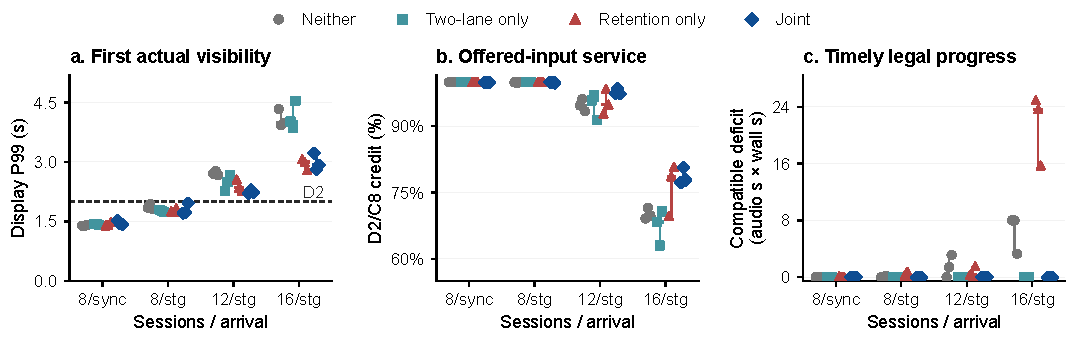
\includegraphics[width=\textwidth]{figures/service_region.pdf}
\caption{All four development workloads and three fresh-process runs per
arm, including the negative twelve-session midpoint. Points are real
per-run values; ticks and ranges describe their median and observed
range. Panel~(c) is the separate secondary measure of subsequent
compatible loss of originally timely intervals, censored at the next
Canonical root when necessary. It does not replace panel~(b)'s original
first-observation credit.}
\label{fig:service-region}
\end{figure*}

All arms pass whole-run D2/C8 in the two eight-session workloads.
Joint display P99 is 1.426--1.528~s when synchronized, where the arms
largely converge. Staggered joint P99 reaches 1.955~s, and an earlier
development run reached 2.034~s, exposing a narrow timing margin.
Two 0.215-s tails exceed D2 in the new eight-session runs and remain
uncredited even though their runs' P99 passes. At sixteen sessions,
all twelve runs fail D2, while C8 passes. Joint credit exceeds $R_0S_0$
by 20.280/22.885/20.180~s, but its credit interactions are
$+20.910$, $+26.380$, and $-9.575$~s.
Against computation-only, joint credit changes by
$+18.910$, $+5.055$, and $-7.225$~s, and display P99 improves
in only one repeat. Continuity is the stable distinction: computation-only
withdraws compatible views 16/17/12 times, versus zero for joint.

First credit does not reveal a later withdrawal. A frozen secondary
recount therefore follows intervals already delivered within D2 whose
eventual certified covering view also meets C8. At each subsequent
Canonical application it classifies withdrawal using the complete old
view's dependency witness, separately recording necessary incompatible
withdrawals. Loss lasts until an actual covering view returns or the
next Canonical boundary censors this root's window. At sixteen sessions,
computation-only still has 10/12/9 timely compatible loss windows with
24.903/23.635/15.736 audio-s$\times$wall-s deficit area; joint has none.
Such holes intersect the original D2 read point for 6.000/10.675/4.000~s
of distinct audio. The secondary measures continuity after delivery;
it neither changes Eq.~\eqref{eq:credit} nor certifies provisional content.

The twelve-session midpoint sought a stronger witness: both
computation-only and joint must pass whole-run D2/C8 in all three
repeats, computation-only must lose an originally timely complete 2-s
non-EOS interval in at least two, and joint must have no compatible
timely loss. This witness is \emph{not established}. All twelve
midpoint runs fail D2; joint P99 is 2.197/2.299/2.228~s.
Computation-only has 1/1/3 timely loss windows, but none qualifies as
a complete non-EOS interval. Joint has zero, yet cannot turn this into
a successful whole-run operating point. The predeclared stop rule
closes this exploration without another session count or extra repeats.

\subsection{Quality and cost boundaries}
All headline Qwen arms have WER $26/1908=1.36\%$ and identical selected
histories. Retrospective support counting first-certified content plus
first-ahead whole views that exactly match later same-$F$ Canonical
text leaves the headline credits unchanged. Elsewhere raw differences
remain: joint loses 2~s of strict support in the sixteen-session third
repeat and 2~s in each of the midpoint's first two repeats, although
the frozen text normalizer agrees. This comparison is with the selected
model output, not human-transcription correctness. Whisper exposes a
larger adapter boundary: WER is 83.12\% at $\rho=1$ and 11.53\% at
$\rho=3$, whose different feedback contract prevents interpreting it
as a quality-preserving speedup.

The headline arms consume similar board energy (Table~\ref{tab:core-h3});
energy does not rank them in credit order. At sixteen development
sessions, joint reduces total model time by 0.66--1.59~s against $R_0S_0$,
while serving wall time does not consistently fall and the
three energy differences change sign. The measured benefit is the
progress delivered and preserved under a fixed feedback contract.
It is not a general reduction in inference cost or a cure for overload.
